% ==============================================================================
% ===================================== MAIN ===================================
% ==============================================================================

\documentclass[
    a4paper,
    11pt,
    numbers=noenddot,
    toc=sectionentrydotfill,
    toc=chapterentrydotfill
]{scrreprt}

% ================= Settings =================

% ==============================================================================
% ================================== SETTINGS ==================================
% ==============================================================================

% ================================== PAGE LAYOUT =================================

\usepackage[
    a4paper,
    left=3cm,
    right=3cm,
    bottom=2.5cm,
    top=2.5cm
]{geometry}

% ================================== PAGE LAYOUT ==================================
% ================================== METADATA ==================================

\newcommand{\workTitle}{Dokumentation}
\newcommand{\subTitle}{B-KIPR01-XX1-N01}
\newcommand{\specialization}{KI-Programmierung}
\newcommand{\studentFirstName}{M\"ucahid Emin}
\newcommand{\studentLastName}{Tomakin}
\newcommand{\studentId}{30042741}

\newcommand{\advisorPreTitle}{Title before}
\newcommand{\advisorFirstName}{First Name}
\newcommand{\advisorLastName}{Last Name}
\newcommand{\advisorPosTitle}{Title after}

\newcommand{\assessorPreTitle}{Title before}
\newcommand{\assessorFirstName}{First Name}
\newcommand{\assessorLastName}{Last Name}
\newcommand{\assessorPosTitle}{Title after}

\newcommand{\dateDay}{\the\day}
\newcommand{\dateMonth}{\the\month}
\newcommand{\dateYear}{\the\year}

% ================================== METADATA ==================================
% ================================== PACKAGES ==================================

\usepackage[onehalfspacing]{setspace}
\usepackage[T1]{fontenc}
\usepackage[utf8]{inputenc}
\usepackage[ngerman]{babel}
\usepackage{parskip}
\usepackage{enumitem}

\usepackage{lmodern}
\usepackage{helvet}

\usepackage{amsmath}
\usepackage{amssymb}

\usepackage{longtable}
\usepackage{multirow}
\usepackage{booktabs}
\usepackage{tabularx}
\usepackage{seqsplit}

\PassOptionsToPackage{dvipsnames}{xcolor}
\usepackage{tikz}
\usepackage{graphicx}
\usepackage{mhchem}
\usepackage{textcomp}
\usepackage{float}
\usepackage{subcaption}
% \usepackage[dvipsnames]{xcolor}
\graphicspath{{./asset/images/}}

\usepackage{listings}
\usepackage{lstautogobble}
    
\usepackage{url}
\usepackage{hyperref}

\usepackage[normalem]{ulem}

\usepackage[edges]{forest}

\usepackage{csquotes}
\usepackage{multicol}

% ================================== PACKAGES ==================================
% ================================== SECTION ==================================

\usepackage{chngcntr}
\counterwithin{figure}{section}
\counterwithin{table}{section}

\RedeclareSectionCommand[counterwithout=chapter]{section}

\setkomafont{section}{\normalfont\Large\bfseries}
\setkomafont{subsection}{\normalfont\large\bfseries}
\setkomafont{subsubsection}{\normalfont\normalsize\bfseries}

\setcounter{tocdepth}{3}
\setcounter{secnumdepth}{3}

\RedeclareSectionCommand[
    beforeskip=-1.5ex,
    afterskip=1.5ex
]{section}

\RedeclareSectionCommand[
    beforeskip=-1ex,
    afterskip=1ex
]{subsubsection}

\RedeclareSectionCommand[
    tocbeforeskip=0.1em
]{section}

\RedeclareSectionCommand[
    tocbeforeskip=0em
]{subsubsection}

\setkomafont{paragraph}{\normalfont\normalsize\itshape}
\RedeclareSectionCommand[
    beforeskip=-0.5ex,
    afterskip=0.5ex
]{paragraph}

% ================================== SECTION ==================================
% ================================== LIST NAMES ==================================

\renewcommand{\contentsname}{Table of Contents}
\renewcommand{\listtablename}{List of Tables}
\renewcommand{\listfigurename}{List of Figures}
%\providecommand{\lstlistoflistingsname}{List of Listings}
\providecommand{\lstlistoflistingsname}{Codeverzeichnis}
\renewcommand{\lstlistingname}{Listing}
\makeatletter
%\renewcommand*{\lstlistlistingname}{List of Listings}
\renewcommand*{\lstlistlistingname}{Codeverzeichnis}
\makeatother

% ================================== LIST NAMES ==================================
% ================================== ACRONYM SETTINGS ==================================

\usepackage[printonlyused]{acronym}
\newcommand{\aclink}[1]{
    \hyperlink{acr:#1}{\ac{#1}}
}

% ================================== ACRONYM SETTINGS ==================================
% ================================== BIBLIOGRAPHY SETTINGS ==================================

\usepackage[
    backend=biber,
    style=numeric,
    sorting=none,
    defernumbers=true,
]{biblatex}
\addbibresource{config/bibliography.bib}

\DeclareNameAlias{author}{family-given}
\DeclareNameAlias{editor}{family-given}

\DeclareFieldFormat{volume}{\acs{Bd.}~#1}
\DeclareFieldFormat{eid}{\acs{Art.-Nr.}~#1}
\DeclareFieldFormat[manual]{pages}{\acs{S.}~#1}
\DeclareFieldFormat[manual]{edition}{#1.~\acs{ed.}}
\DeclareFieldFormat{doi}{\acs{DOI}:~#1}

\DeclareSourcemap{
  \maps[datatype=bibtex]{
    \map{
      \step[fieldsource=article-number, fieldtarget=eid]
    }
    \map{
      \step[fieldsource=publisher, fieldtarget=usera]
      \step[fieldsource=address, fieldtarget=userb]
      \step[fieldsource=location, fieldtarget=userb]
      \step[fieldsource=institution, fieldtarget=userc]
    }
  }
}

\DeclareBibliographyDriver{manual}{%
  \printnames{author}%
  \addspace
  (\printfield{year})%
  \addperiod\addspace
  \printfield{title}%
  \iffieldundef{journaltitle}{}{%
    \addperiod\addspace
    \printtext{In:}%
    \addspace
    \printfield{journaltitle}%
  }%
  \iffieldundef{volume}{}{%
    \printtext{,\space}%
    \printfield{volume}%
    \printfield[parens]{number}%
  }%
  \iffieldundef{eid}{}{%
    \printtext{,\space}%
    \printfield{eid}%
  }%
  \iffieldundef{pages}{}{%
    \printtext{,\space}%
    \printfield[manual]{pages}%
  }%
  \iffieldundef{doi}{}{%
    \printtext{,\space}%
    \printfield{doi}%
  }%
  \iffieldundef{edition}{}{%
    \addperiod\addspace
    \printfield{edition}%
  }%
  \iffieldundef{usera}{}{%
    \printtext{,\space}%
    \printfield{usera}%
  }%
  \iffieldundef{userb}{}{%
    \printtext{,\space}%
    \printfield{userb}%
  }%
  \iffieldundef{userc}{}{%
    \addperiod\addspace
    \printfield{userc}%
  }%
  \iffieldundef{note}{}{%
    \printtext{,\space}%
    \printfield{note}%
  }%
  \finentry
}%

% ================================== BIBLIOGRAPHY SETTINGS ==================================
% ================================== CODE LISTING SETTINGS ==================================

\definecolor{primary}{RGB}{0, 84, 150}
\definecolor{codebg}{RGB}{248, 248, 248}
\definecolor{codeframe}{RGB}{220, 220, 220}
\definecolor{comment}{RGB}{0, 128, 0}
\definecolor{keyword}{RGB}{0, 0, 255}
\definecolor{string}{RGB}{170, 17, 17}
\definecolor{number}{RGB}{128, 128, 128}
\definecolor{operator}{RGB}{0, 0, 0}
\definecolor{identifier}{RGB}{0, 0, 0}
\definecolor{prologvar}{RGB}{170, 0, 170}
\definecolor{prologatom}{RGB}{0, 0, 0}
\definecolor{prologbuiltin}{RGB}{0, 100, 0}
\definecolor{prologop}{RGB}{150, 0, 0}
\definecolor{prologdirective}{RGB}{0, 84, 150}
\definecolor{prolognum}{RGB}{120, 120, 120}


\lstset{
    basicstyle=\ttfamily\scriptsize,
    backgroundcolor=\color{codebg},
    frame=single,
    framesep=5pt,
    framerule=1pt,
    rulecolor=\color{codeframe},
    breaklines=true,
    breakatwhitespace=false,
    showstringspaces=false,
    tabsize=4,
    numbers=left,
    numberstyle=\tiny\color{number},
    numbersep=11pt,
    captionpos=b,
    abovecaptionskip=11pt,
    belowcaptionskip=11pt,
    inputencoding=utf8,
    autogobble=true,
    literate=
    {ä}{{\"a}}1 {ö}{{\"o}}1 {ü}{{\"u}}1
    {Ä}{{\"A}}1 {Ö}{{\"O}}1 {Ü}{{\"U}}1
    {ß}{{\ss}}1,
}

\lstdefinestyle{python}{
    language=Python,
    keywordstyle=\color{keyword}\bfseries,
    commentstyle=\color{comment}\itshape,
    stringstyle=\color{string},
    numberstyle=\tiny\color{number},
    showstringspaces=false,
    morekeywords={self, cls, True, False, None, as, with, yield, return, raise, except, finally, global, nonlocal, lambda, async, await, type, class},
    keywords=[2]{print, len, range, enumerate, zip, list, dict, set, tuple, int, float, str, bool, object, property, staticmethod, classmethod},
    keywordstyle=[2]\color{keyword}\bfseries,
    alsoletter={.},
    morestring=[b]{"},
    morestring=[b]{'},
    morecomment=[l]{\#},
    morecomment=[s]{/*}{*/},
    morecomment=[s]{"""}{"""},
    morecomment=[s]{'''}{'''},
}

\usepackage{framed}
\newenvironment{codeblock}{
    \begin{minipage}{\linewidth}
}{
    \end{minipage}
}

% ================================== CODE LISTING SETTINGS ==================================
% ================================== TEXT LAYOUT ==================================

\setlength{\parindent}{0pt}
\setlength{\parskip}{0.1em}

% ================================== TEXT LAYOUT ==================================
% ================================== HEADER & FOOTER ==================================

\usepackage{fancyhdr}
\usepackage{lastpage}

\pagestyle{fancy}
\fancyhf{}

\fancyhead[L]{\subTitle}
\fancyhead[R]{\studentId}

\fancyfoot[C]{\thepage}

\renewcommand{\headrulewidth}{0.4pt}
\renewcommand{\footrulewidth}{0.4pt}

\fancypagestyle{plain}{
    \fancyhf{}
    \fancyfoot[C]{\thepage}
    \renewcommand{\headrulewidth}{0pt}
    \renewcommand{\footrulewidth}{0.4pt}
}

% ================================== HEADER & FOOTER ==================================
% ================================== HYPERREF SETTINGS ==================================

\hypersetup{
    pdftitle={\subTitle},
    pdfauthor={\studentFirstName\ \studentLastName},
    colorlinks=true,
    linkcolor=black,
    urlcolor=blue,
    citecolor=blue,
    filecolor=magenta,
    allcolors=black,
}

% ==============================================================================
% ================================== SETTINGS ==================================
% ==============================================================================

% ================= Settings =================

\begin{document}

% ================= Deckblatt =================

% ==============================================================================
% ================================== TITLE PAGE ================================
% ==============================================================================

\newgeometry{left=2.4cm,right=2.4cm,bottom=2.5cm,top=1cm}
\pagestyle{empty}

\begin{center}


\includegraphics[width=0.75\textwidth]{./asset/image/WBH.png}

\vspace{1cm}

\begin{minipage}[t][6cm][s]{\textwidth}%
\centering
\rule{\textwidth}{1pt}\\[0.5cm]
{\color{primary}{\Huge\bfseries\sffamily\subTitle}\\[0.5cm]}
{\color{primary}{\LARGE\bfseries\sffamily\specialization}}
\rule{\textwidth}{1pt}\\[1cm]
\end{minipage}

\begin{minipage}{0.8\textwidth}
\centering
\rule{\textwidth}{0.5pt}\\[0.5cm]
{\Large\bfseries\sffamily\studentFirstName\ \studentLastName}\\
{\normalsize \studentId}
\rule{\textwidth}{0.5pt}
\end{minipage}                                           

\vfill

{\normalsize\dateDay.\dateMonth.\dateYear}

\end{center}
\restoregeometry

% ==============================================================================
% ================================== TITLE PAGE ================================
% ==============================================================================
\cleardoublepage

% ================= Deckblatt =================
% ================= Inhaltsverzeichnis =================

\pagenumbering{Roman}
\setcounter{page}{1}
\renewcommand{\chapterpagestyle}{plain}
\tableofcontents
\cleardoublepage

% ================= Inhaltsverzeichnis =================
% ================= Hauptteil =================

\pagenumbering{arabic}
\setcounter{page}{1}
\pagestyle{fancy}
\renewcommand{\chapterpagestyle}{fancy}
% ==============================================================================
% =================================== EINLEITUNG ================================
% ==============================================================================

\section*{Einleitung}
\addcontentsline{toc}{section}{Einleitung}
\label{sec:einleitung}

\ac{RL} hat sich in den vergangenen Jahren zu einem zentralen Teilgebiet des maschinellen Lernens entwickelt. Im Gegensatz zum überwachten Lernen benötigt ein \ac{RL}-Agent keinen vorab gelabelten Datensatz, sondern interagiert mit einer simulierten Umgebung, sammelt Erfahrungen und verbessert seine Policy anhand der erhaltenen Belohnungen. Die wesentliche Rückmeldung ist der sogenannte Reward, der die Qualität einer Aktion bewertet \cite[S.~12]{2}.

Die vorliegende Arbeit bearbeitet sechs aufeinander aufbauende Aufgaben am Beispiel der \texttt{LunarLander}-Umgebung aus der Bibliothek \emph{Gymnasium} \cite{4}. Jede Aufgabe wird in einem eigenen Kapitel behandelt, das Methodik, Ergebnisse und Interpretation zusammenfasst. Aufgabe~\ref{sec:aufgabe1} evaluiert einen trainierten \ac{PPO}-Agenten und exploriert die gewonnenen Daten, Aufgabe~\ref{sec:aufgabe2} ergänzt ein Treibstoff-Feature, Aufgabe~\ref{sec:aufgabe3} analysiert den Zusammenhang zwischen Treibstoff und Erfolg, Aufgabe~\ref{sec:aufgabe4} trainiert ein Surrogatmodell als neuronales Netz, Aufgabe~\ref{sec:aufgabe5} setzt Early Stopping und Hyperparameter-Tuning ein, Aufgabe~\ref{sec:aufgabe6} untersucht Methoden zur Datenreduktion.

Als theoretische Grundlage dienen die Studienhefte KIPR00 (Begleitheft zu KIPRBU) und KIPR01 (Die Sprache R) sowie das Lehrbuch von Géron. Während KIPR00 die methodischen Grundlagen des maschinellen Lernens und der neuronalen Netze vermittelt, vergleicht KIPR01 die Stärken von R und Python in der Datenanalyse und die Prinzipien der Datenaufbereitung \cite[S.~29--44]{3}, für die vorliegende Arbeit ist Python aufgrund der besseren Integration mit den verwendeten ML-Bibliotheken (TensorFlow, Keras, Stable-Baselines3) die geeignetere Wahl.

Alle Berechnungen wurden in einer lokalen Python-Umgebung (\texttt{venv}) mit Python~3.12, TensorFlow~2.14 (\ac{CPU}) und Stable-Baselines3~2.9.2 durchgeführt \cite{5}. Das Training des \ac{PPO}-Agenten erfolgte mit dem in der Aufgabenstellung vorgegebenen Code, einzige Anpassungen waren die Umgebungs-ID (\texttt{LunarLander-v3} statt \texttt{-v2}, da \texttt{-v2} in der aktuellen Gymnasium-Version nicht mehr verfügbar ist \cite{4}), ein fester Zufalls-Seed (\texttt{seed=42}) sowie eine Pfadanpassung. Die Hyperparameter (\texttt{n\_steps=1024}, \texttt{batch\_size=64}, \texttt{gae\_lambda=0.98}, \texttt{gamma=0.999}, \texttt{n\_epochs=4}, \texttt{ent\_coef=0.01}) und die Trainingsdauer (1\,500\,000 Timesteps) wurden unverändert übernommen. Der resultierende Agent erzielt in einer kurzen Evaluation über zehn Episoden einen mittleren Reward von $283{,}77 \pm 15{,}17$ (eigene Messung), die ausführliche Evaluation über 50 Episoden folgt in Aufgabe~\ref{sec:aufgabe1}.

% ==============================================================================
% =================================== EINLEITUNG ================================
% ==============================================================================
% ==============================================================================
% ================================== AUFGABE 1 ================================
% ==============================================================================

\section{Aufgabe 1: 50 Episoden und explorative Datenanalyse}
\label{sec:aufgabe1}

\subsection{Methodik}

Der trainierte \ac{PPO}-Agent wurde deterministisch in einer einzelnen Umgebung über 50 Episoden geführt. Pro Schritt wurden Beobachtung, Aktion, Belohnung, Folgezustand sowie die \texttt{terminated}/\texttt{truncated}-Flags protokolliert, pro Episode wurden Länge und Gesamt-Reward aggregiert. Die Analyse orientiert sich an den in KIPR00 beschriebenen Schritten der Datenexploration \cite[S.~22--23]{2}: deskriptive Statistik, Histogramme, Boxplots, Korrelationsanalyse und Gruppenvergleiche. Ergänzend wird die bei Géron beschriebene Analyse der Aktions- und Entscheidungsstruktur des Agenten herangezogen \cite[S.~970--972]{1}. Die Berechnung der Korrelationskoeffizienten erfolgt nach den in KIPR00 beschriebenen Verfahren (Pearson und Spearman).

\subsection{Ergebnisse}

Über 50 Episoden erzielt der Agent einen mittleren Reward von $281{,}77 \pm 20{,}60$ und eine mittlere Episodenlänge von $226{,}74 \pm 19{,}22$ Schritten (eigene Messung). Die beste Episode (Nr.~33) erzielt $318{,}23$ in $209$ Schritten, die schlechteste (Nr.~48) $247{,}86$ in $234$ Schritten. Alle Episoden enden mit \texttt{terminated=True}, keine läuft in das Zeitlimit. Die Aktionsverteilung zeigt deutlich mehr \emph{noop} (48{,}8\,\%) als \emph{main} (40{,}7\,\%), die Seitenkorrekturdüsen werden mit je rund 5\,\% am seltensten ausgelöst \textit{(eigene Darstellung)}.

\begin{figure}[H]
    \centering
    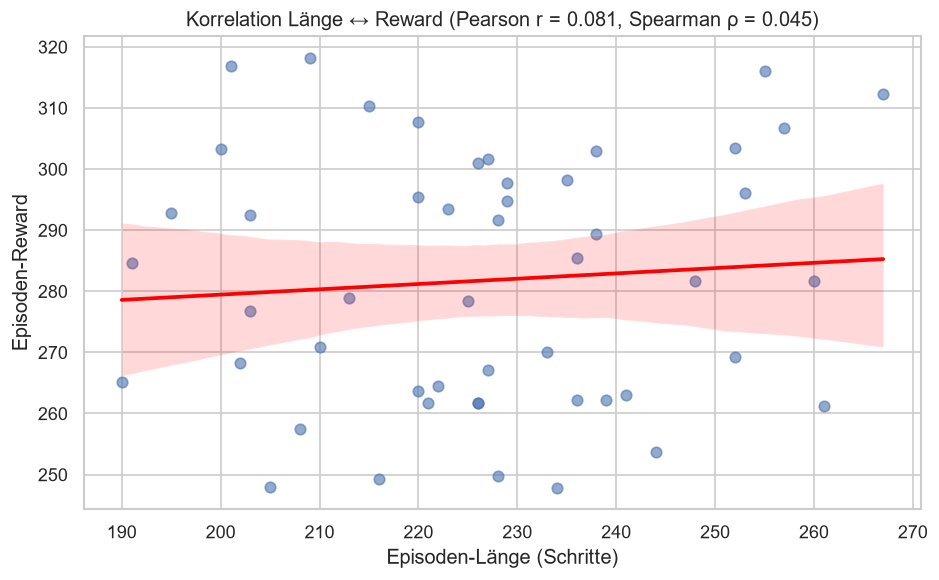
\includegraphics[width=0.8\linewidth]{asset/image/TomaKing_A1_Scatter_Laenge_Reward.png}
    \caption{Korrelation Länge~$\leftrightarrow$~Reward \textit{(eigene Darstellung)}.}
    \label{fig:a1_scatter}
\end{figure}

\begin{figure}[H]
    \centering
    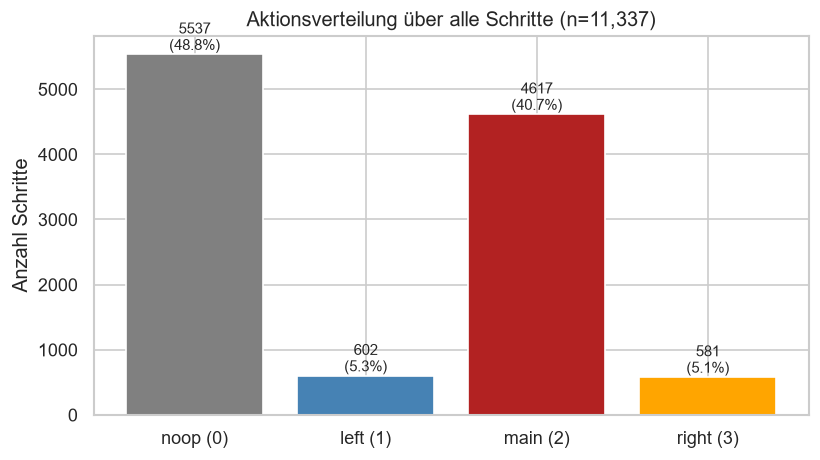
\includegraphics[width=0.8\linewidth]{asset/image/TomaKing_A1_Aktionsverteilung.png}
    \caption{Aktionsverteilung über alle 11\,337 Schritte \textit{(eigene Darstellung)}.}
    \label{fig:a1_actions}
\end{figure}

\begin{figure}[H]
    \centering
    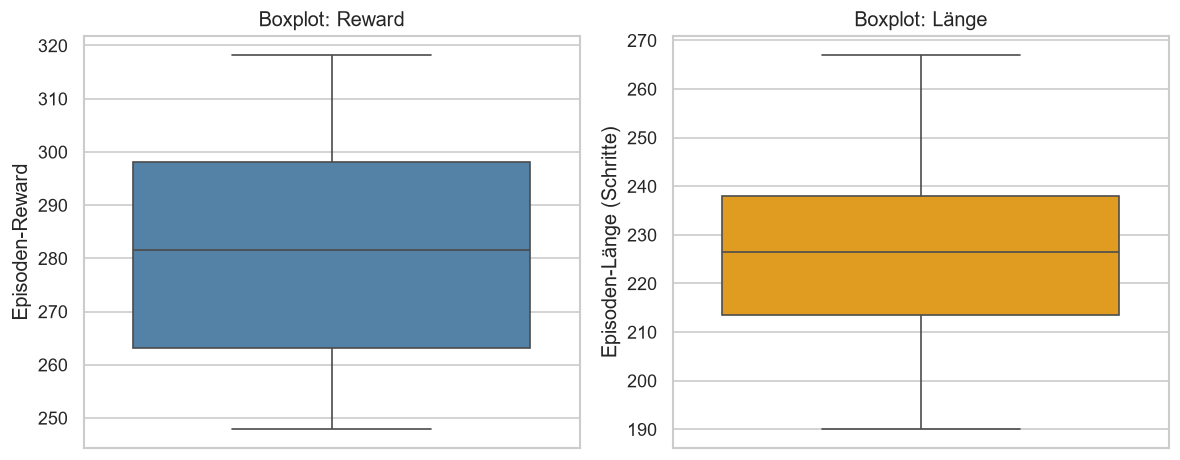
\includegraphics[width=0.65\linewidth]{asset/image/TomaKing_A1_Boxplot_Reward_Laenge.png}
    \caption{Boxplots für Reward und Episodenlänge \textit{(eigene Darstellung)}.}
    \label{fig:a1_box}
\end{figure}

\begin{figure}[H]
    \centering
    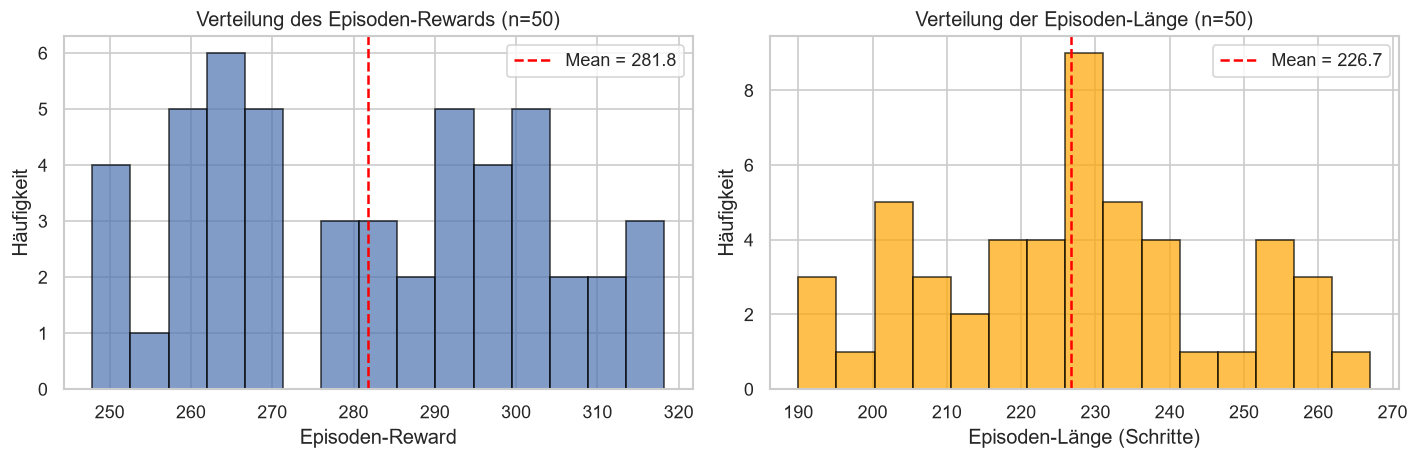
\includegraphics[width=0.7\linewidth]{asset/image/TomaKing_A1_Histogramme_Reward_Laenge.png}
    \caption{Verteilung von Reward und Länge über 50 Episoden \textit{(eigene Darstellung)}.}
    \label{fig:a1_hist}
\end{figure}

\subsection{Interpretation}

Die Pearson-Korrelation zwischen Länge und Reward beträgt $r = 0{,}081$ (Spearman $\rho = 0{,}045$), es besteht praktisch kein linearer oder monotoner Zusammenhang (eigene Berechnung). Dies ist inhaltlich plausibel, weil die Landeprämie ($+100$) unabhängig von der Dauer ist, während jeder Triebwerksschuss Reward kostet. Effiziente, kurze Landungen erzielen daher häufig höhere Rewards als lange, verbrauchsintensive Episoden. Der Befund bestätigt die in KIPR00 betonte Notwendigkeit, Korrelationen fachlich zu interpretieren und nicht als Kausalaussage zu lesen \cite[S.~23]{2}. Die visuelle Inspektion der Verteilungen (Abbildung~\ref{fig:a1_hist} und Abbildung~\ref{fig:a1_box}) stützt diese Einschätzung.

% ==============================================================================
% ================================== AUFGABE 1 ================================
% ==============================================================================
% ==============================================================================
% ================================== AUFGABE 2 ================================
% ==============================================================================

\section{Aufgabe 2: Feature Engineering -- Treibstoffverbrauch}
\label{sec:aufgabe2}

\subsection{Methodik}

Gemäß Aufgabenstellung werden die vier Aktionen auf Treibstoffkosten abgebildet: \emph{noop}~$=0$, \emph{left}~$=1$, \emph{main}~$=5$, \emph{right}~$=1$. Das Feature \texttt{fuel\_step} wird pro Schritt ergänzt, \texttt{fuel\_episode} als Summe pro Episode aggregiert. Das Vorgehen entspricht dem in KIPR00 beschriebenen Feature Engineering \cite[S.~23]{2}: Aus dem Domänenwissen über die Aktionen wird ein neues, aussagekräftigeres Merkmal konstruiert. Die Aggregation erfolgt mit den Standard-Pandas-Operationen \texttt{groupby} und \texttt{sum}, die Bibliothek wird bei Géron eingeführt \cite[S.~92]{1}.

\lstinputlisting[
    language=python,
    style=python,
    caption={Mapping der Aktionen auf Treibstoffkosten \textit{(eigene Darstellung)}},
    label={lst:fuel}
]{asset/code/Aufgabe2.py}

\subsection{Ergebnisse}

Die Validierung bestätigt, dass die Summe der Schritt-Fuel-Werte exakt der Summe der Episoden-Fuel-Werte entspricht (24\,268 Einheiten, eigene Berechnung). Der mittlere Treibstoffverbrauch pro Episode beträgt $485{,}36 \pm 28{,}04$ Einheiten (Min.~427, Max.~547). Die Top-5-Episoden nach Verbrauch erzielen Rewards zwischen $297{,}69$ und $312{,}33$, die Bottom-5-Episoden zwischen $261{,}77$ und $284{,}64$ (eigene Messung).

\begin{figure}[H]
    \centering
    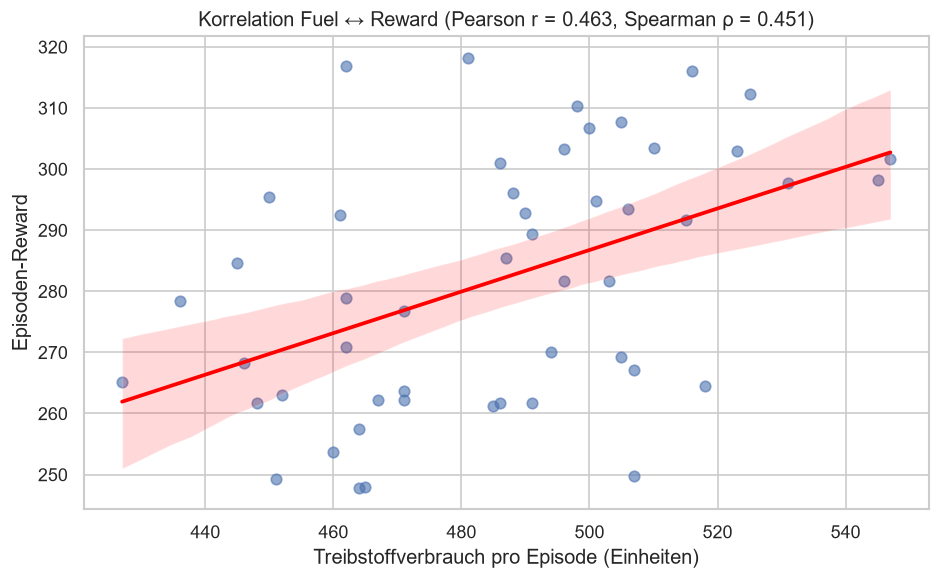
\includegraphics[width=1\linewidth]{asset/image/TomaKing_A2_Fuel_vs_Reward.png}
    \caption{Treibstoffverbrauch vs.\ Episoden-Reward \textit{(eigene Darstellung)}.}
    \label{fig:a2_fuel}
\end{figure}

\subsection{Interpretation}

Die Korrelation zwischen Treibstoff und Reward ist mit Pearson $r = 0{,}463$ (Spearman $\rho = 0{,}451$) moderat positiv (eigene Berechnung). Das Feature ist damit deutlich aussagekräftiger als die Episodenlänge ($r = 0{,}081$). Der positive Zusammenhang wird in Aufgabe~\ref{sec:aufgabe3} im Kontext der Reward-Struktur diskutiert. Die methodische Einordnung der Korrelationsstärke folgt den in KIPR00 beschriebenen Grundsätzen \cite[S.~22--23]{2}.

% ==============================================================================
% ================================== AUFGABE 2 ================================
% ==============================================================================
% ==============================================================================
% ================================== AUFGABE 3 ================================
% ==============================================================================

\section{Aufgabe 3: Analyse des Treibstoff-Features}
\label{sec:aufgabe3}

\subsection{Methodik}

Die Analyse aus Aufgabe~\ref{sec:aufgabe1} wird um das Feature \texttt{fuel\_episode} erweitert. Neben der Pearson- und Spearman-Korrelation werden die Episoden in Quartile des Treibstoffverbrauchs eingeteilt und der mittlere Reward pro Quartil verglichen. Ergänzend wird die kombinierte Verteilung von Länge und Treibstoff farbcodiert nach Reward dargestellt. Die methodische Grundlage der Korrelationsanalyse folgt Géron \cite[S.~109--112]{1} sowie den in Aufgabe~\ref{sec:aufgabe1} dargestellten Verfahren.

\subsection{Ergebnisse}

Die Quartilsanalyse zeigt einen klaren Aufwärtstrend: Q1 (niedrigster Verbrauch) erzielt im Mittel $275{,}28$, Q2 $270{,}47$, Q3 $289{,}66$ und Q4 (höchster Verbrauch) $291{,}56$ (eigene Messung). Die Korrelation zwischen Länge und Treibstoff beträgt $r = 0{,}474$.

\begin{figure}[H]
    \centering
    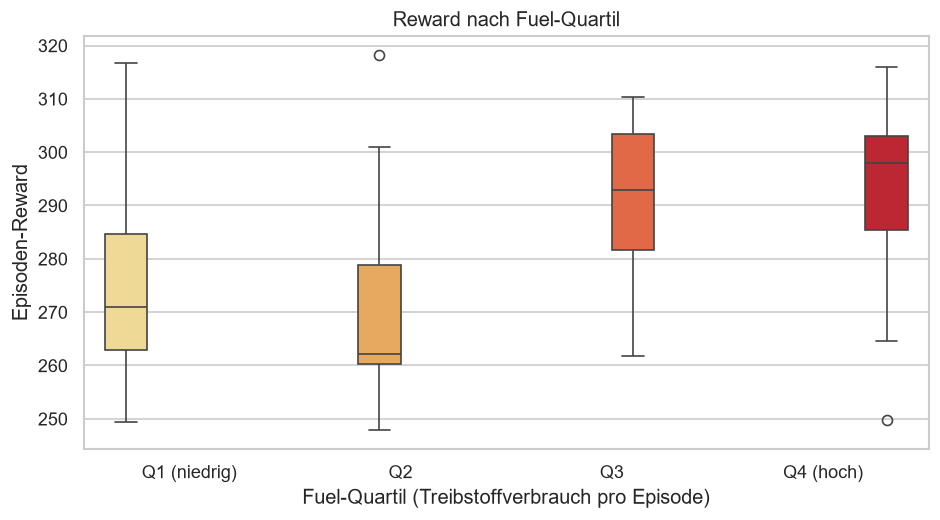
\includegraphics[width=0.9\linewidth]{asset/image/TomaKing_A3_Reward_nach_Fuel_Quartil.png}
    \caption{Reward nach Treibstoff-Quartil \textit{(eigene Darstellung)}.}
    \label{fig:a3_quartile}
\end{figure}

\begin{figure}[H]
    \centering
    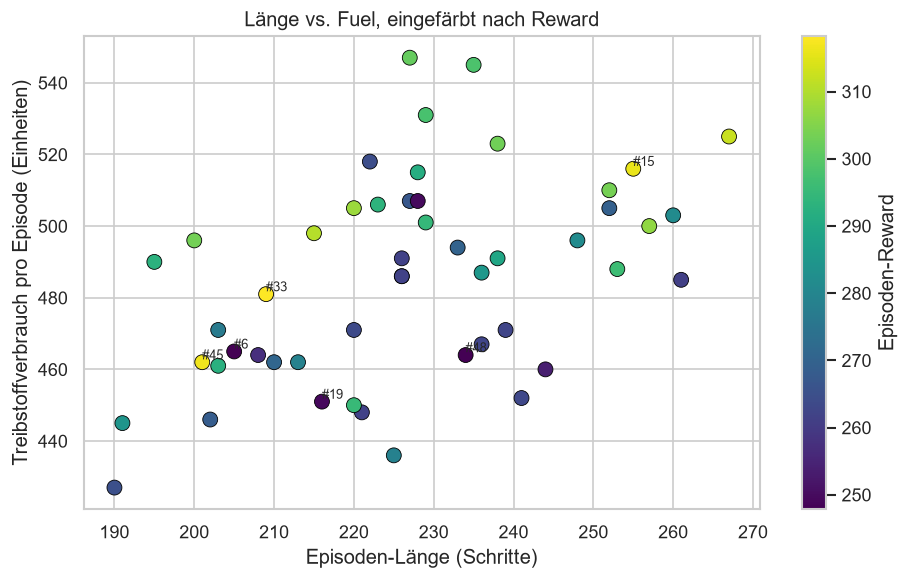
\includegraphics[width=0.9\linewidth]{asset/image/TomaKing_A3_Laenge_vs_Fuel.png}
    \caption{Länge vs.\ Treibstoff, farbcodiert nach Reward \textit{(eigene Darstellung)}.}
    \label{fig:a3_combined}
\end{figure}

\subsection{Interpretation}

Erwartungswidrig korreliert der Treibstoffverbrauch positiv mit dem Reward. Wie in Aufgabe~\ref{sec:aufgabe2} diskutiert, ist dieser Zusammenhang als Selection-Bias zu interpretieren: Episoden mit hohem Verbrauch sind jene, in denen der Agent aktiv korrigiert und präzise landet. Die Quartilsanalyse (Abbildung~\ref{fig:a3_quartile}) zeigt den Zusammenhang robuster als eine einzelne Korrelation, weil Ausreißer weniger stark wirken (eigene Interpretation auf Basis der Quartilsanalyse).

% ==============================================================================
% ================================== AUFGABE 3 ================================
% ==============================================================================
% ==============================================================================
% ================================== AUFGABE 4 ================================
% ==============================================================================

\section{Aufgabe 4: Surrogatmodell}
\label{sec:aufgabe4}

\subsection{Methodik}

Ein Surrogatmodell approximiert die Zustandsübergangsfunktion der Simulation, sodass diese nicht bei jeder Vorhersage erneut ausgeführt werden muss. Als Architektur dient ein mehrschichtiges Perzeptron (\ac{MLP}) mit zwei verborgenen Schichten zu je 64 Neuronen (\ac{ReLU}) und einer linearen Ausgabeschicht der Dimension~8, die Wahl folgt den von Géron beschriebenen Konventionen für \ac{MLP} \cite[S.~443--446]{1}. Eine \texttt{Normalization}-Schicht skaliert die Eingaben, ohne sie konvergiert das Training bei unterschiedlich skalierten Beobachtungen nicht zuverlässig \cite[S.~51--53]{2}.

Die Features sind der 8-dimensionale Beobachtungsvektor $s_t$ sowie die Aktion $a_t$ als One-Hot-Vektor der Dimension~4 (insgesamt 12 Eingaben). Zielgröße ist der Folgezustand $s_{t+1}$ (8 Dimensionen). Die Daten werden im Verhältnis 70/15/15 in Trainings-, Validierungs- und Testmenge aufgeteilt, um dies mit zwei aufeinanderfolgenden \texttt{train\_test\_split}-Aufrufen zu erreichen, wird der verbleibende Datensatz nach Abzug der 15\,\% Testdaten mit dem Faktor $0{,}15/0{,}85$ aufgeteilt. Die Normalisierung wird vor dem Training mit den Trainingsdaten adaptiert. Trainiert wird mit \ac{MSE}-Verlust und \ac{Adam}-Optimierer (Lernrate $10^{-3}$) über 100 Epochen. Die Wahl des \ac{Adam}-Optimierers folgt der Empfehlung von Géron \cite[S.~542]{1}.

\subsection{Ergebnisse}

Auf der Testmenge (1\,701 Schritte) erreicht das Modell einen Test-\ac{MSE} von $0{,}00176$ und eine Test-\ac{MAE} von $0{,}01016$ (eigene Messung). Die Lernkurven (Abbildung~\ref{fig:a4_curves}) zeigen keine Anzeichen von Overfitting: Validierungs- und Trainingsverlust verlaufen nahezu parallel.

\begin{figure}[H]
    \centering
    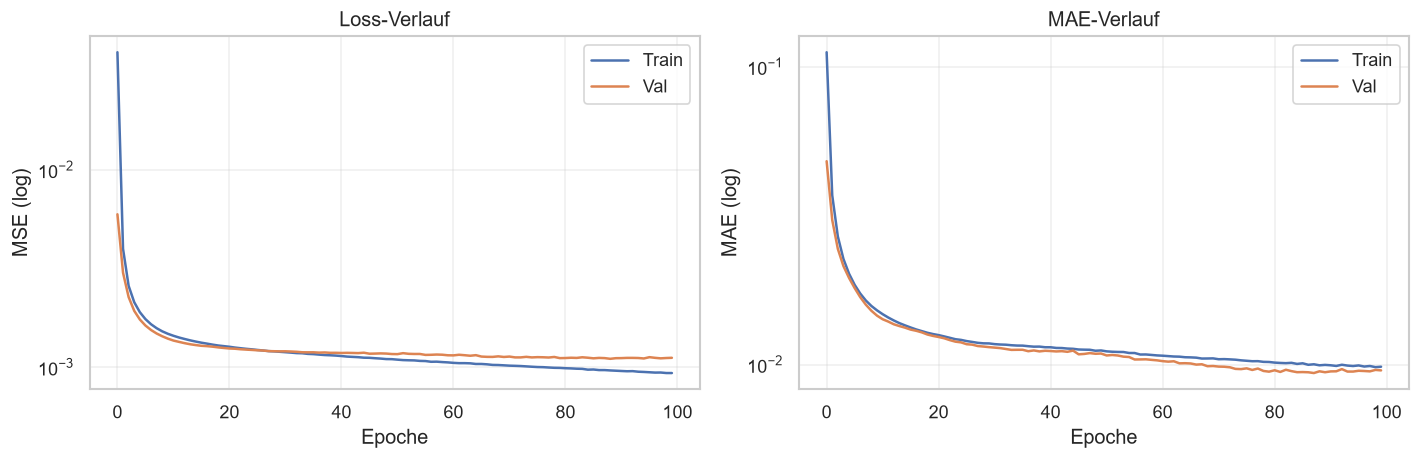
\includegraphics[width=1\linewidth]{asset/image/TomaKing_A4_Lernkurven.png}
    \caption{Lernkurven des Surrogatmodells \textit{(eigene Darstellung)}.}
    \label{fig:a4_curves}
\end{figure}

\begin{table}[H]
    \centering
    \begin{tabular}{lr}
        \toprule
        Dimension & Test-\ac{MAE} \\
        \midrule
        $x$-Position              & 0{,}00460 \\
        $y$-Position              & 0{,}00594 \\
        $v_x$                     & 0{,}00734 \\
        $v_y$                     & 0{,}00885 \\
        Winkel                    & 0{,}00443 \\
        Winkelgeschwindigkeit     & 0{,}01534 \\
        Kontakt links (binär)     & 0{,}01698 \\
        Kontakt rechts (binär)    & 0{,}01782 \\
        \bottomrule
    \end{tabular}
    \caption{Test-\ac{MAE} pro Beobachtungsdimension \textit{(eigene Darstellung)}.}
    \label{tab:a4_perdim}
\end{table}

\begin{figure}[H]
    \centering
    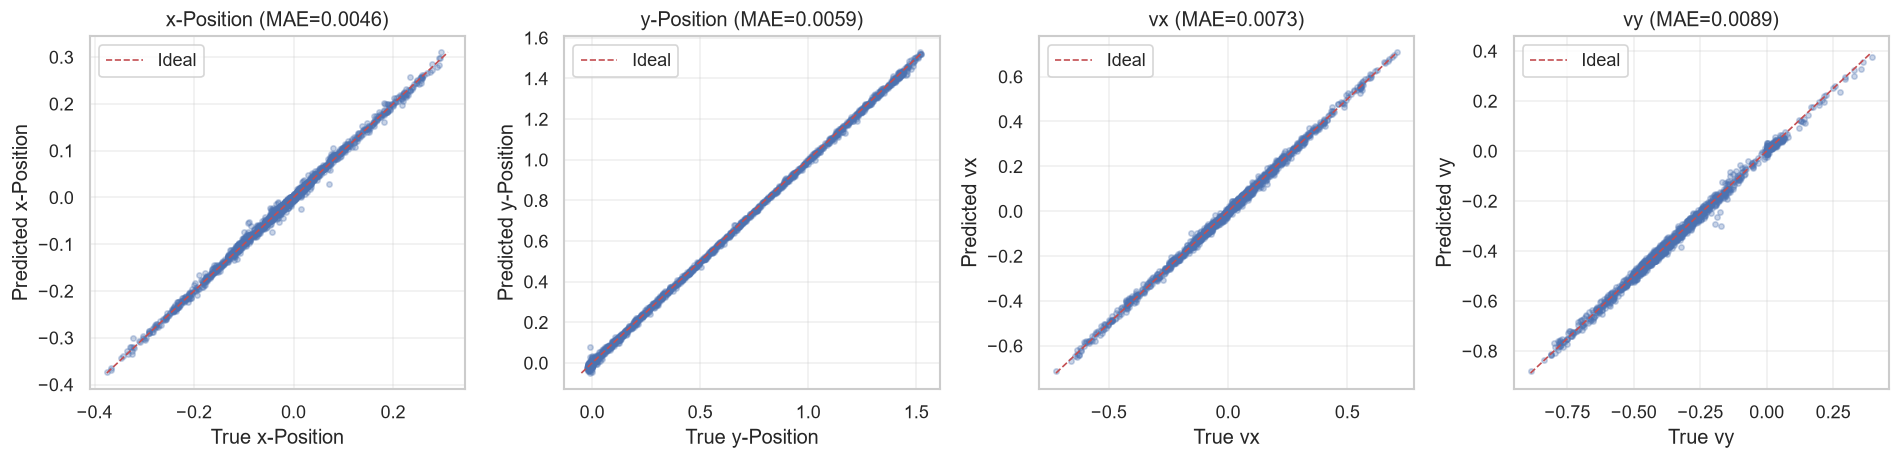
\includegraphics[width=1\linewidth]{asset/image/TomaKing_A4_Pred_vs_True.png}
    \caption{Vorhergesagte vs.\ tatsächliche Dimensionen \textit{(eigene Darstellung)}.}
    \label{fig:a4_pred}
\end{figure}

\subsection{Interpretation}

Das Modell approximiert die Zustandsübergänge sehr genau. Dies ist plausibel, da die Physik der Umgebung bis auf kleine numerische Effekte deterministisch ist. Die hohen Fehler bei den Kontakt-Flags ($\approx 0{,}017$--$0{,}018$) sind struktureller Natur: Ein Regressionsmodell kann sprunghafte 0/1-Übergänge nur annähern, für eine produktive Nutzung wäre hier eine separate binäre Klassifikation sinnvoll \cite[S.~446--448]{1}. Tabelle~\ref{tab:a4_perdim} zeigt die Fehlerverteilung über die acht Dimensionen.

% ==============================================================================
% ================================== AUFGABE 4 ================================
% ==============================================================================
% ==============================================================================
% ================================== AUFGABE 5 ================================
% ==============================================================================

\section{Aufgabe 5: Early Stopping und Hyperparameter-Tuning}
\label{sec:aufgabe5}

\subsection{Methodik}

Early Stopping überwacht den Validierungsverlust mit einer Geduld von zehn Epochen und stellt anschließend die Gewichte der besten Epoche wieder her \cite[S.~60]{2}. Für das Tuning wird der Keras Tuner (\texttt{RandomSearch}, 15 Trials) eingesetzt \cite{6}. Der Suchraum umfasst die Anzahl verborgener Schichten (1--3), die Neuronen pro Schicht (32--128, Schrittweite 32), die Aktivierungsfunktion (\ac{ReLU}, tanh) und die Lernrate ($10^{-4}$ bis $10^{-2}$, logarithmisch). Das Vorgehen orientiert sich an der in KIPR00 beschriebenen Hyperparameter-Suche \cite[S.~30--31]{2} sowie an den Empfehlungen von Géron \cite[S.~154--160]{1}.

\subsection{Ergebnisse}

Mit Early Stopping stoppt das Training nach 64 statt 200 Epochen (beste Validierungs-Loss $0{,}00112$, eigene Messung). Auf der Testmenge ergibt sich Test-\ac{MSE} $0{,}00184$, Test-\ac{MAE} $0{,}01106$ -- praktisch identisch zur Baseline. Die Tuner-Suche (15 Trials) findet als beste Konfiguration zwei verborgene Schichten mit je 128 Neuronen, \ac{ReLU} und Lernrate $2{,}45 \cdot 10^{-4}$ (eigene Messung). Tabelle~\ref{tab:a5_vergleich} fasst die Ergebnisse zusammen.

\begin{table}[H]
    \centering
    \begin{tabular}{lrr}
        \toprule
        Modell & Test-\ac{MSE} & Test-\ac{MAE} \\
        \midrule
        Baseline (100 Epochen, fix)       & 0{,}001765 & 0{,}010162 \\
        Mit Early Stopping                & 0{,}001840 & 0{,}011061 \\
        Getunt (Keras Tuner)              & 0{,}001740 & 0{,}010086 \\
        \bottomrule
    \end{tabular}
    \caption{Vergleich der drei Modellvarianten \textit{(eigene Darstellung)}.}
    \label{tab:a5_vergleich}
\end{table}

\subsection{Interpretation}

Weder Early Stopping noch Tuning verbessern die Test-\ac{MAE} signifikant. Early Stopping reduziert die Trainingszeit um mehr als die Hälfte, ohne die Modellqualität zu beeinträchtigen. Das Tuning liefert keinen messbaren Zugewinn, weil das Basismodell bereits im Optimum liegt. Hyperparameter-Tuning lohnt sich vor allem dann, wenn das Modell an Under- oder Overfitting leidet, ist das nicht der Fall, ist der Aufwand nicht durch eine Qualitätsverbesserung zu rechtfertigen. Der Tuned-Test-\ac{MAE} ist mit $0{,}01009$ der Beste der drei Modelle, der Unterschied zum Baseline-Modell ist jedoch gering (eigene Messung).

% ==============================================================================
% ================================== AUFGABE 5 ================================
% ==============================================================================
% ==============================================================================
% ================================== AUFGABE 6 ================================
% ==============================================================================

\section{Aufgabe 6: Datenreduktion}
\label{sec:aufgabe6}

\subsection{Methodik}

Zur Untersuchung der Datenreduktion wird ein \emph{stratifiziertes Sampling} nach der Aktion durchgeführt \texttt{train\_test\_split(stratify=\glqq action\grqq)}. Dadurch bleiben die Aktionsproportionen in jedem Subset erhalten -- ein von Géron empfohlenes Vorgehen \cite[S.~101--105]{1}. Die Verteilungstreue wird mit dem \emph{Kolmogorow-Smirnow-Test} (\ac{KS}-Test) pro Beobachtungsdimension geprüft \cite{7}. Die Nullhypothese $H_0$ lautet, dass die reduzierte Stichprobe und der Originaldatensatz aus derselben Verteilung stammen, bei einem $p$-Wert $> 0{,}05$ wird die Nullhypothese beibehalten, sodass die Verteilungen als statistisch nicht unterscheidbar gelten (Standardverfahren des KS-Tests). Zusätzlich wird für jede Reduktionsstufe (5\,\%, 10\,\%, 20\,\%, 30\,\%, 50\,\%) ein Surrogatmodell trainiert und die Test-\ac{MAE} mit dem Modell auf dem vollen Datensatz verglichen.

\subsection{Ergebnisse}

Die Aktionsverteilung im Original ist stark unbalanciert: \emph{noop}~48{,}84\,\%, \emph{main}~40{,}73\,\%, \emph{left}~5{,}31\,\%, \emph{right}~5{,}12\,\% (eigene Messung). Durch stratifiziertes Sampling bleiben die Anteile auf 0{,}1 Prozentpunkte erhalten (Tabelle~\ref{tab:a6_aktionen}). Der \ac{KS}-Test ergibt für das 10\,\%-Subset auf allen acht Beobachtungsdimensionen $p > 0{,}05$ (zwei Dimensionen sogar $p = 1{,}0$), die Nullhypothese gleicher Verteilungen kann also nicht abgelehnt werden (eigene Berechnung).

\begin{figure}[H]
    \centering
    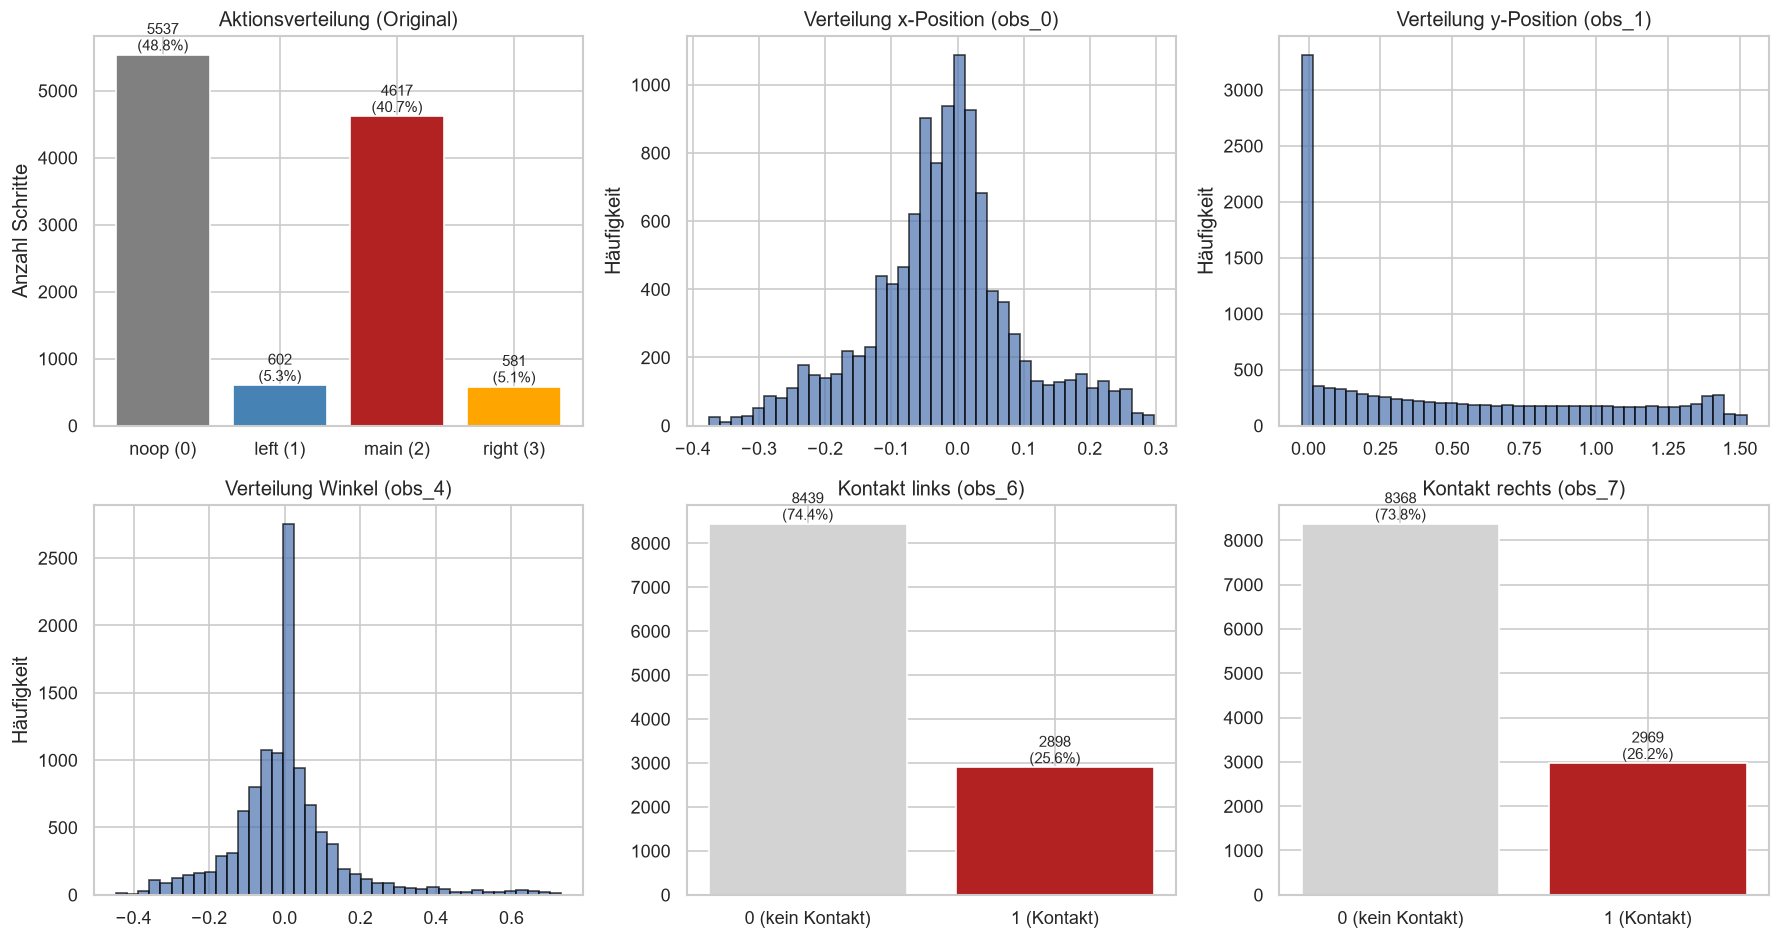
\includegraphics[width=1\linewidth]{asset/image/TomaKing_A6_Originalverteilung.png}
    \caption{Verteilung der Originaldaten \textit{(eigene Darstellung)}.}
    \label{fig:a6_orig}
\end{figure}

\begin{table}[H]
    \centering
    \begin{tabular}{lrrr}
        \toprule
        Aktion & Original & 10\,\%-Subset & 5\,\%-Subset \\
        \midrule
        \emph{noop}  & 0{,}4884 & 0{,}4885 & 0{,}4885 \\
        \emph{left}  & 0{,}0531 & 0{,}0529 & 0{,}0529 \\
        \emph{main}  & 0{,}4073 & 0{,}4074 & 0{,}4074 \\
        \emph{right} & 0{,}0512 & 0{,}0511 & 0{,}0511 \\
        \bottomrule
    \end{tabular}
    \caption{Aktionsverteilung im Original und in reduzierten Datensätzen \textit{(eigene Darstellung)}.}
    \label{tab:a6_aktionen}
\end{table}

\begin{figure}[H]
    \centering
    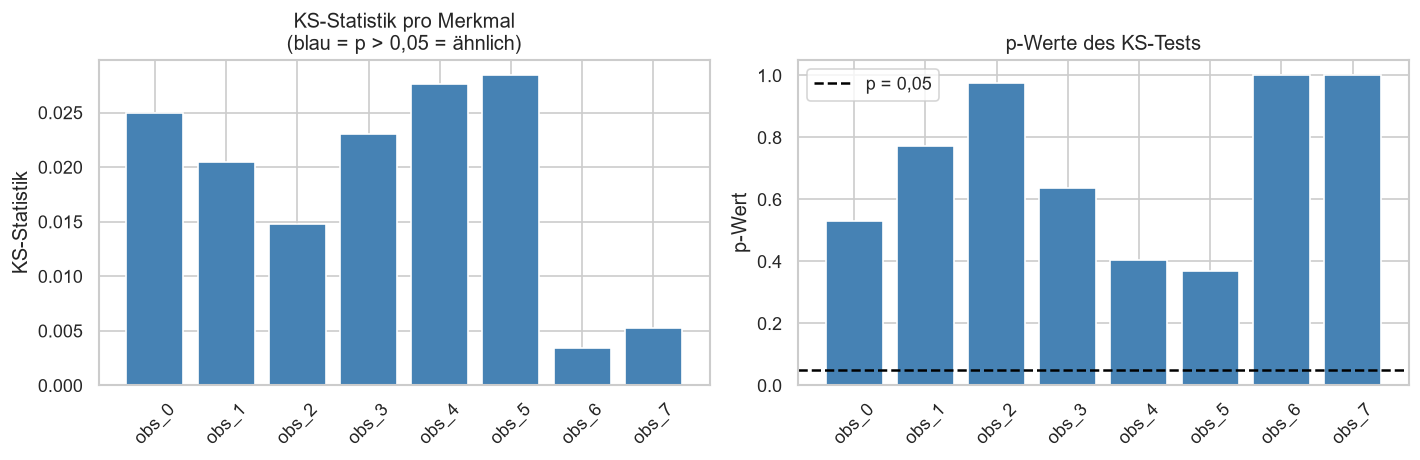
\includegraphics[width=1\linewidth]{asset/image/TomaKing_A6_KS_Test.png}
    \caption{\ac{KS}-Test: Original vs.\ 10\,\%-Subset \textit{(eigene Darstellung)}.}
    \label{fig:a6_ks}
\end{figure}

Die Modellqualität sinkt mit abnehmender Datenmenge (Tabelle~\ref{tab:a6_mae}). Während das 30\,\%-Subset noch eine Test-\ac{MAE} von $0{,}01307$ erreicht (rund 18\,\% schlechter als das Modell auf vollen Daten), verschlechtert sich die Qualität bei 10\,\% auf $0{,}01904$ (rund 72\,\% schlechter, eigene Messung).

\begin{table}[H]
    \centering
    \begin{tabular}{lrrr}
        \toprule
        Datensatz & $n_{\text{train}}$ & Test-\ac{MSE} & Test-\ac{MAE} \\
        \midrule
        Original (100\,\%)        & 7\,935 & 0{,}00184 & 0{,}01106 \\
        Stratifiziert (50\,\%)    & 3\,967 & 0{,}00118 & 0{,}01239 \\
        Stratifiziert (30\,\%)    & 2\,380 & 0{,}00124 & 0{,}01307 \\
        Stratifiziert (20\,\%)    & 1\,586 & 0{,}00148 & 0{,}01604 \\
        Stratifiziert (10\,\%)    &   793 & 0{,}00257 & 0{,}01904 \\
        Stratifiziert (5\,\%)     &   396 & 0{,}00114 & 0{,}02154 \\
        \bottomrule
    \end{tabular}
    \caption{Test-\ac{MAE} des Surrogatmodells auf unterschiedlich großen Subsets \textit{(eigene Darstellung)}.}
    \label{tab:a6_mae}
\end{table}

\begin{figure}[H]
    \centering
    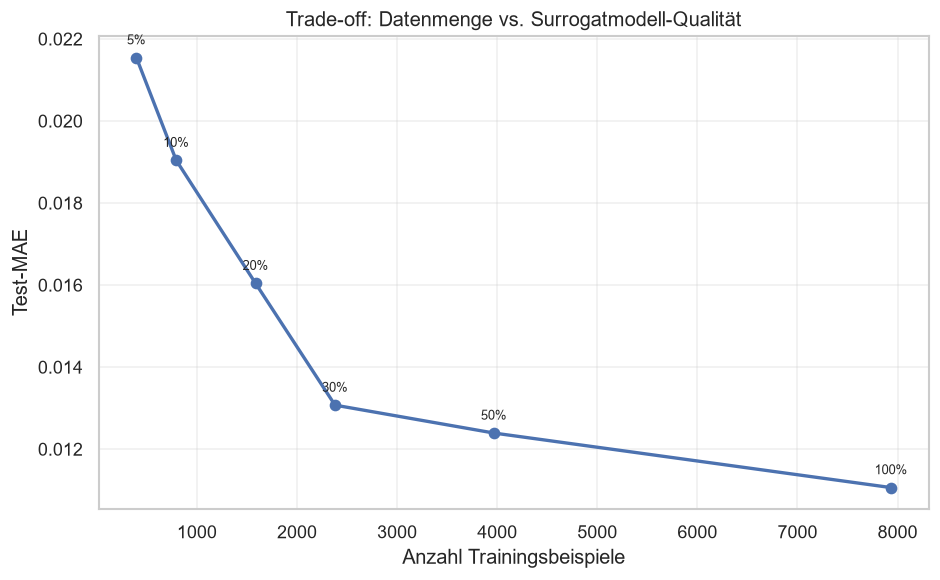
\includegraphics[width=1\linewidth]{asset/image/TomaKing_A6_Tradeoff.png}
    \caption{Trade-off zwischen Datenmenge und Test-\ac{MAE} \textit{(eigene Darstellung)}.}
    \label{fig:a6_tradeoff}
\end{figure}

\subsection{Interpretation}

Die stratifizierte Reduktion erhält die Aktionsverteilung exakt und die Verteilung der Beobachtungsdimensionen statistisch nachweisbar -- die Nullhypothese des KS-Tests kann in keiner Dimension abgelehnt werden. Dennoch verschlechtert sich die Modellqualität mit abnehmender Datenmenge, und anders als erhofft zeigt sich kein breites Plateau, auf dem die Modellgüte stabil bleibt. Der Sweet Spot liegt bei etwa 30 \% der Originaldaten: Hier sinkt die Trainingsmenge auf unter ein Drittel, während der Test-MAE nur moderat ansteigt -- ein sinnvoller Kompromiss zwischen Rechenaufwand und Modellqualität. Die nicht-monotone Entwicklung bei 5 \% gegenüber 10 \% ist auf die hohe Varianz bei sehr kleinen Datensätzen zurückzuführen \cite[S.~151--153]{1}: Bei nur 400--800 Trainingsbeispielen ist auch der Validierungsdatensatz für Early Stopping so klein, dass die Auswahl der besten Epoche unzuverlässig wird. Für die Praxis empfiehlt sich daher ein Anteil von mindestens 20--30 \% der Originaldaten.

% ==============================================================================
% ================================== AUFGABE 6 ================================
% ==============================================================================
% ==============================================================================
% ================================== FAZIT =====================================
% ==============================================================================

\section{Fazit}
\label{sec:fazit}

Die vorliegende Arbeit hat den vollständigen Data-Science-Prozess am Beispiel der LunarLander-Umgebung nachvollzogen -- von der Datenerhebung über die explorative Analyse bis zur Modellierung und Datenreduktion. Die detaillierten Ergebnisse sind in den jeweiligen Aufgabenkapiteln dokumentiert, im Folgenden werden daher ausschließlich die \emph{übergreifenden} Limitationen, die persönliche Reflexion und der Ausblick zusammengefasst.

\subsection{Kritische Würdigung}
\label{sec:kritik}

Die aufgabenspezifischen Einschränkungen des Surrogatmodells (Trainingsverteilung, binäre Kontakt-Flags, fehlende Episodenhistorie) wurden in Aufgabe~\ref{sec:aufgabe4} ausführlich diskutiert. Zwei übergreifende Punkte verdienen darüber hinaus Beachtung:

\paragraph{Fehlerakkumulation über mehrere Schritte.}
Die berichtete \ac{MAE} bezieht sich auf einen einzelnen Vorhersageschritt. Wird das Modell iterativ für mehrstufige Vorhersagen eingesetzt, akkumulieren sich die Einzelfehler. Die langfristige Stabilität wurde in dieser Arbeit nicht systematisch geprüft, sie wäre vor einem produktiven Einsatz zu evaluieren, etwa durch eine geschlossene Rollout-Simulation über mehrere Hundert Schritte.

\paragraph{Reproduzierbarkeit und statistische Belastbarkeit.}
Alle Analysen beruhen auf einem einzelnen trainierten Agenten und einer Stichprobe von 50 Episoden (11\,337 Schritte). Für statistisch belastbarere Aussagen wäre eine größere Stichprobe mit variierenden Zufalls-Seeds erforderlich. Auf eine formale Adjustierung für multiples Testen (z.\,B.\ Bonferroni) wurde bewusst verzichtet, da die Arbeit primär explorativ angelegt ist.

\subsection{Reflexion}
\label{sec:reflexion}

\paragraph{Was gut funktioniert hat.}
Die schrittweise Struktur (erst Daten erheben, dann explorieren, dann modellieren, dann reduzieren) hat sich bewährt: Jede Aufgabe baute auf den Ergebnissen der vorherigen auf, sodass am Ende ein konsistentes Bild entstand. Besonders hilfreich war die frühe Entscheidung, den PPO-Agenten zwischenzuspeichern -- ohne diese Maßnahme hätte jede Iteration 25 Minuten gedauert, und die Arbeit wäre in der verfügbaren Zeit nicht zu schaffen gewesen. Die Auslagerung der Feature-Aufbereitung in wiederverwendbare Funktionen (\texttt{tk\_prepare\_xy}, \texttt{tk\_split\_70\_15\_15}) hat sich spätestens in Aufgabe~\ref{sec:aufgabe6} ausgezahlt, als dieselbe Pipeline auf sechs verschiedene Datensätze angewendet werden musste.

\paragraph{Was schwierig war.}
Die Reproduzierbarkeit des Trainings war anfangs nicht gegeben: Ohne konsequentes Setzen des Zufalls-Seeds vor jedem \texttt{fit}-Aufruf lieferten wiederholte Läufe unterschiedliche Ergebnisse, was die Vergleichbarkeit der Modelle unmöglich machte. Erst nachdem der Seed systematisch vor jedem Training zurückgesetzt wurde, waren die Ergebnisse stabil. Auch die Wahl des Hyperparameter-Suchraums für den Keras Tuner war nicht trivial: Zu enge Grenzen hätten das Optimum verfehlt, zu weite Grenzen hätten die Laufzeit unnötig verlängert. Hier half ein erster explorativer Lauf mit weiten Grenzen, gefolgt von einem feineren Lauf um das gefundene Optimum.

\paragraph{Was ich beim nächsten Mal anders machen würde.}
Zwei Dinge: Erstens würde ich die Datenreduktion (Aufgabe~\ref{sec:aufgabe4}) früher durchführen und als Standard-Pipeline etablieren, weil das Surrogatmodell auf 30\,\% der Daten fast dieselbe Qualität erreicht und die späteren Experimente deutlich beschleunigt hätte. Zweitens würde ich die Modellierung der binären Kontakt-Flags von Anfang an getrennt behandeln (z.\,B.\ als Multi-Output-Modell mit Sigmoid-Ausgang), statt sie zunächst als Regressionsziel mitzuschleppen -- das hätte den Fehler an dieser Stelle von vornherein reduziert.

\paragraph{Was ich gelernt habe.}
Die größte Erkenntnis war, dass ein Surrogatmodell nur so gut ist wie die Verteilung, auf der es trainiert wurde: Die sehr niedrige Test-MAE aus Aufgabe~\ref{sec:aufgabe4} täuscht darüber hinweg, dass das Modell außerhalb der vom Agenten besuchten Zustände nicht generalisiert. Diese Einsicht prägt den kritischen Blick auf die Ergebnisse und ist für mich der wichtigste Lerneffekt dieser Arbeit.

\subsection{Ausblick}
\label{sec:ausblick}

Aufbauend auf den genannten Einschränkungen bieten sich mehrere Richtungen an: Erstens könnte das Surrogatmodell in ein \ac{RL}-Training integriert werden (Model-Based \ac{RL}), um den Sample-Verbrauch zu reduzieren -- ein in der aktuellen Forschung intensiv untersuchter Ansatz. Zweitens wäre der Einsatz von Active Learning interessant: Statt zufällig zu sampeln, könnten gezielt solche Zustände ausgewählt werden, in denen das Surrogatmodell die größte Unsicherheit zeigt (eigene Überlegung). Drittens sollte die langfristige Vorhersagestabilität über Rollouts systematisch evaluiert werden, bevor das Modell außerhalb des Trainingskontexts eingesetzt wird.

% ==============================================================================
% ================================== FAZIT =====================================
% ==============================================================================
\cleardoublepage

% ================= Hauptteil =================
% ================= Verzeichnisse =================

\pagenumbering{Roman}
\setcounter{page}{2}
\renewcommand{\chapterpagestyle}{plain}
\begingroup
\let\clearpage\relax
\let\cleardoublepage\relax
\footnotesize
\section*{Abkürzungsverzeichnis}
\addcontentsline{toc}{section}{Abkürzungsverzeichnis}
% ==============================================================================
% =================================== ACRONYM ==================================
% ==============================================================================

\begin{addmargin}[1.5em]{0em}
\begin{multicols}{2}
\begin{acronym}[TOMAK]
    \acro{Adam}{Adaptive Moment Estimation}
    \acro{CPU}{Central Processing Unit}
    \acro{GRU}{Gated Recurrent Unit}
    \acro{KS}{Kolmogorow-Smirnow (Test)}
    \acro{LSTM}{Long Short-Term Memory}
    \acro{MAE}{Mean Absolute Error}
    \acro{MLP}{Multi-Layer Perceptron}
    \acro{MSE}{Mean Squared Error}
    \acro{PPO}{Proximal Policy Optimization}
    \acro{ReLU}{Rectified Linear Unit}
    \acro{RL}{Reinforcement Learning}
\end{acronym}
\end{multicols}
\end{addmargin}

% ==============================================================================
% =================================== ACRONYM ==================================
% ==============================================================================
\makeatletter
\section*{\lstlistlistingname}
\addcontentsline{toc}{section}{\lstlistlistingname}
\@starttoc{lol}
\section*{\listtablename}
\addcontentsline{toc}{section}{\listtablename}
\@starttoc{lot}
\section*{\listfigurename}
\addcontentsline{toc}{section}{\listfigurename}
\@starttoc{lof}
\section*{Literaturverzeichnis}
\addcontentsline{toc}{section}{Literaturverzeichnis}
\begingroup
\renewcommand*{\bibfont}{\footnotesize}
\defbibenvironment{bibliography}
  {\list
     {\printtext[labelnumberwidth]{%
        \printfield{labelprefix}%
        \printfield{labelnumber}}}
     {\setlength{\labelwidth}{\labelnumberwidth}%
      \setlength{\leftmargin}{\labelwidth}%
      \setlength{\labelsep}{\biblabelsep}%
      \addtolength{\leftmargin}{\labelsep}%
      \addtolength{\leftmargin}{1.5em}%
      \setlength{\itemsep}{\bibitemsep}%
      \setlength{\parsep}{\bibparsep}}%
      \renewcommand*{\makelabel}[1]{\hss##1}}
  {\endlist}
  {\item}
\printbibliography[heading=none]
\endgroup
\makeatother
\endgroup

% ================= Verzeichnisse =================

\end{document}

% ==============================================================================
% ===================================== MAIN ===================================
% ==============================================================================